\documentclass[11pt, reqno]{amsart}

\usepackage[spanish]{babel}
\usepackage[LGR, T1]{fontenc}
\usepackage[utf8]{inputenc}

../LaTeX/general.tex
% \input{../graphics.tex}

\makeatletter
\def\emailaddrname{\textit{Correo electrónico}}
\def\subtitle#1{\gdef\@subtitle{#1}}
\def\@subtitle{}

% Metadata
\def\logo#1{\gdef\@logo{#1}}
\def\@logo{}
\def\institution#1{\gdef\@institution{#1}}
\def\@institution{}
\def\department#1{\gdef\@department{#1}}
\def\@department{}
\def\professor#1{\gdef\@professor{#1}}
\def\@professor{}
\def\course#1{\gdef\@course{#1}}
\def\@course{}
\def\coursecode#1{\gdef\@coursecode{#1}}
\def\@coursecode{}

\renewcommand{\maketitle}{
\begin{center}
	\small
	\renewcommand{\arraystretch}{1.2}
	\begin{tabular}{cp{.37\textwidth}p{0.44\textwidth}}
		% \hline
		\multirow{5}{*}{\includegraphics[height=2.0cm]{\@logo}}
	  & \multicolumn{2}{c}{ \makecell{{\bfseries \@institution} \\ \@department} } \\
	  % & \multicolumn{2}{c|}{{\bfseries\@institution} \\ \@department} \\
	  \cline{2-3}
	  & \textbf{Profesor:} \@professor & \textbf{Ayudante:} \authors \\
	  % \cline{2-3}
	  & \textbf{Curso:} \@course & \textbf{Sigla:} \@coursecode \\
	  % \cline{2-3}
	  & \multicolumn{2}{l}{ \textbf{Fecha:} \@date } \\
	  % \hline
	\end{tabular}
	\\[\baselineskip]
	% {}
	% \vspace{2\baselineskip}
	{\bfseries\Large\@title}
	\ifx\@subtitle\@empty\else
		\\[1ex]
		\large\mdseries\@subtitle
	\fi
\end{center}
}
\makeatother

\usepackage{multirow, makecell}

\usepackage[
	reversemp,
	letterpaper,
	% marginpar=2cm,
	% marginsep=1pt,
	margin=2.3cm
]{geometry}
\usepackage{fontawesome}
% \makeatletter
% \@reversemargintrue
% \makeatother

% Símbolos al margen, necesitan doble compilación
\newcommand{\hard}{\marginnote{\faFire}}
\newcommand{\hhard}{\marginnote{\faFire\faFire}}

% Dependencias para los teoremas
\usepackage{xifthen}
\def\@thmdep{}
\newcommand{\thmdep}[1]{
	\ifthenelse{\isempty{#1}}
	{\def\@thmdep{}}
	{\def\@thmdep{ (#1)}}
}
\newcommand{\thmstyle}{\color{thm}\sffamily\bfseries}

% ===== Estilos de Teoremas ==========
\newtheoremstyle{axiomstyle}
	{0.3cm}
	{0.3cm}
	{\normalfont}
	{0.5cm}
	{\bfseries\scshape}
	{:}
	{4pt}
	{\thmname{#1}\thmnote{ #3}\thmnumber{ (#2)}}
\newtheoremstyle{styleC}
	{0.5cm}
	{0.5cm}
	{\normalfont}
	{0.5cm}
	{\bfseries}
	{:}
	{4pt}
	{\thmname{#1\textrm{\@thmdep}}\thmnumber{ #2}\thmnote{ (#3)}}

% ====== Teoremas (sin borde) ===========
\theoremstyle{axiomstyle}
\newtheorem*{axiom}{Axioma}

% ====== Teoremas (sin borde) ==================
\theoremstyle{styleC}
\newtheorem{thm}{Teorema}[section]
\newtheorem{mydef}[thm]{Definición}
\newtheorem{prop}[thm]{Proposición}
\newtheorem{cor}[thm]{Corolario}
\newtheorem{lem}[thm]{Lema}
\newtheorem{con}[thm]{Conjetura}

\newtheorem*{prob}{Problema}
\newtheorem*{sol}{Solución}
\newtheorem*{obs}{Observación}
\newtheorem*{ex}{Ejemplo}

% \usepackage{tcolorbox}
% \newtcbox{bluebox}[1][]{enhanced jigsaw, 
%   sharp corners,
%   frame hidden,
%   nobeforeafter,
%   listing only,
%   #1} % comando para crear cajas de colores

\expandafter\let\expandafter\oldproof\csname\string\proof\endcsname
\let\oldendproof\endproof
\renewenvironment{proof}[1][\proofname]{%
  \oldproof[\scshape Demostración:]%
}{\oldendproof} % comando para redefinir la caja de la demostración
\newenvironment{hint}[1][\proofname]{%
  \oldproof[\scshape Pista:]%
}{\oldendproof} % comando para redefinir la caja de la demostración

% colores utilizados
\definecolor{numchap}{RGB}{249,133,29}
\definecolor{chap}{RGB}{6,129,204}
\definecolor{sec}{RGB}{204,0,0}
\definecolor{thm}{RGB}{106,176,240}
\definecolor{thmB}{RGB}{32,31,31}
\definecolor{part}{RGB}{212,66,66}

% ====== Diseño de los titulares ===============
\usepackage[explicit]{titlesec} % para personalizar el documento, la opción <<explicit>> hace que el texto de los titulares sea un objeto interactuable

\titleformat{\subsection}[runin]
	{\bfseries}
	{\textrm{\S}\thesubsection}
	{1ex}
	{#1.}

\setlist[enumerate,1]{label=\arabic*., ref=\arabic*} % Enumerate standards

% \usepackage{diagbox}

\title{Enteros gaussianos}
\subtitle{Diofanto contraataca}
\date{12 de octubre de 2023}

\author[José Cuevas]{José Cuevas Barrientos}
\email{josecuevasbtos@uc.cl}

\logo{../puc_negro.png}
\institution{Pontificia Universidad Católica de Chile}
\department{Facultad de Matemáticas}
\course{Teoría de Números}
\coursecode{MAT2225}
\professor{Héctor Pastén}

\begin{document}

\maketitle

\section{Los enteros gaussianos}
\begin{lem}
	Sea $d \in \Z$ un entero cualquiera.
	Entonces
	\[
		A := \Z[\sqrt{d}] = \{ a + b\sqrt{d} : a, b \in \Z \}
	\]
	es un anillo (i.e., cerrado bajo suma y producto).
\end{lem}
Nótese que la proposición anterior permite construir anillos más grandes eligiendo $d$ más pequeño.
Por ejemplo, $\Z[ \sqrt{n^2 m} ] \subseteq \Z[ \sqrt{m} ]$.

\begin{mydef}
	Sobre el anillo $A := \Z[\sqrt{d}]$, donde $d$ no es un cuadrado, se definen la función \strong{conjugado} $\overline{()} \colon A \to A$
	y la función \strong{norma} $\galnorm\colon A \to \Z$ dadas por
	\[
		\overline{a + b\sqrt{d}} := a - b\sqrt{d}, \qquad \galnorm(a + b\sqrt{d}) := (a + b\sqrt{d}) \overline{(a + b\sqrt{d})} = a^2 - db^2.
	\]
	Los elementos del anillo $\Z[\sqrt{-1}]$ se dicen \strong{enteros gaussianos}.
	Denotaremos $\ui := \sqrt{-1}$.
\end{mydef}
\begin{thm}\label{thm:gauss_is_euclid}
	Los enteros gaussianos forman un dominio euclidiano con la norma y, por lo tanto, es un dominio de factorización única (DFU).
\end{thm}
Recuérdese que un dominio íntegro $A$ se dice euclidiano si existe una función $\phi \colon A_{\ne 0} \to \N$ para todo par $\alpha, \beta \in A$
con $\beta \ne 0$ existen $\gamma, \delta$ tales que $\alpha = \beta \gamma + \delta$, donde $\delta$ o bien es cero, o bien $\phi(\delta) < \phi(\beta)$.
\begin{proof}
	Sean $\alpha, \beta \in A := \Z[\ui]$ con $\beta \ne 0$.
	Podemos identificar a $\alpha, \beta \in \C$ y así $\alpha/\beta =: \theta \in \C$ es un número complejo.
	Mirando el retículo $A = \Z + \ui\Z \subseteq \C$ notamos que siempre existe $\gamma \in A$ tal que $|\theta - \gamma|$ es <<pequeño>>,
	para ser más precisos, $|\theta - \gamma| \le \sqrt{2}/2$ (ver fig.~\ref{fig:gauss_int}).
	\begin{figure}[!hbt]
		\centering
		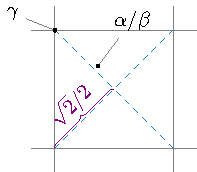
\includegraphics[scale=1]{../gauss_int.pdf}
		\caption{}%
		\label{fig:gauss_int}
	\end{figure}

	Así que definiendo $\delta := \beta(\theta - \gamma)$, tenemos la siguiente igualdad:
	$$ \alpha = \beta \theta = \beta \gamma + \delta, $$
	donde $\delta = \alpha - \beta \gamma \in A$ puesto que $A$ es un anillo, y donde $|\delta| < |\beta|\cdot\sqrt{2}/2 < |\beta|$.
	Finalmente, nótese que la norma realmente es $\galnorm(a + b\ui) = a^2 + b^2 = |a + b\ui|^2$, de modo que $\galnorm(\delta) < \galnorm(\beta)$
	como se quería probar.
\end{proof}

Cuando un anillo es un DFU tenemos la gran ventaja de que un elemento es irreducible syss es primo, de modo que se entiende la factorización
conociendo las unidades y los primos.
\begin{prop}
	Sea $d$ un entero que no es un cuadrado y sea $A := \Z[\sqrt{d}]$.
	Se cumplen:
	\begin{enumerate}
		\item La conjugación $\overline{()} \colon A \to A$ es un isomorfismo de anillos.
		\item Para todo $\alpha, \beta \in A$ se cumple que $\galnorm(\alpha \beta) = \galnorm(\alpha) \, \galnorm(\beta)$.
		\item Un elemento $\alpha \in A$ es una unidad syss $\galnorm(\alpha) \in \{ \pm 1 \}$.
		\item Si $\alpha \in A$ es tal que $\galnorm(\alpha)$ es primo, entonces $\alpha$ es irreducible en $A$.
	\end{enumerate}
\end{prop}
\begin{proof}
	\begin{enumerate}
		\item Basta  notar que $\overline{()}$ respeta sumas y productos, puesto que es claramente biyectivo.
		\item $\galnorm(\alpha \beta) = \alpha \, \overline{\alpha} \cdot \beta \, \overline{\beta} = \alpha \beta \cdot \overline{\alpha \beta}
			= \galnorm(\alpha) \, \galnorm(\beta)$.
		\item $\implies$. Si $\alpha$ tiene inversa $\gamma := \alpha^{-1}$, entonces
			\[
				\galnorm(\alpha) \galnorm(\gamma) = \galnorm(\alpha \gamma) = \galnorm(1) = 1,
			\]
			así que $\galnorm(\alpha)$ es una unidad de $\Z$, es decir, es $\pm 1$.

			$\impliedby$. Como $\alpha \overline{\alpha} = \galnorm(\alpha) = \pm 1$, entonces $\pm\overline{\alpha} = \alpha^{-1}$.
		\item Por contrarrecíproca, si $\alpha = \beta \gamma$, donde $\beta, \gamma$ no son invertibles, entonces
			$\galnorm(\alpha) = \galnorm(\beta) \galnorm(\gamma)$ y $\galnorm(\beta), \galnorm(\gamma)$ no son unidades de $\Z$,
			así que $\galnorm(\alpha)$ es compuesto. \qedhere
	\end{enumerate}
\end{proof}
El criterio del inciso 4 no es una equivalencia.
Por ejemplo, es fácil probar que 2 es irreducible en $\Z[\sqrt{3}]$, pero $\galnorm(2) = 4$.

De estudiar la ecuación $\galnorm(a + b\ui) = a^2 + b^2 = \pm 1$ se sigue que:
\begin{cor}
	$\Z[\ui]^\times = \{ \pm 1, \pm \ui \}$.
\end{cor}
Para tener control total sobre la factorización en un anillo es necesario conocer los primos, pero también las unidades.
Nótese que esta es una ventaja de que el $d$ sea negativo; cuando el $d$ es positivo, la condición de la norma nos dice que las
unidades vienen dadas por la solución a unas ecuaciones de Pell, por lo tanto tendrán infinitas unidades.

\section{Dos ecuaciones diofantinas}
\begin{thm}
	Las únicas soluciones enteras de la ecuación $y^2 = x^3 - 4$ son
	$$ (x, y) \in \{ (2, \pm 2), (5, \pm 11) \}. $$
\end{thm}
\begin{proof}
	Reescribamos $x^3 = 4 + y^2 = (2 - \ui y)(2 + \ui y)$.
	\begin{itemize}
		\item \underline{Si $y$ es impar:}
			Notamos que un divisor común $\alpha$ de $2 - \ui y$ y $2 + \ui y$ es divisor común de su suma 4
			y por lo tanto $\galnorm(\alpha) \mid 16$ y $\galnorm(\alpha) \mid x^3$.
			Si $y$ es impar, entonces $x$ también y luego $\alpha = 1$, por lo que son coprimos.
			Luego ambos factores son cubos en $\Z[\ui]$ y aplicando conjugados comprobamos:
			$$ 2 + \ui y = (a + \ui b)^3, \qquad 2 - \ui y = (a - \ui b)^3, $$
			restando ambas expresiones, e igualando partes imaginarias, se obtiene que
			$$ 4 = 2b(b^2 - 3a^2) \iff 2 = b(b^2 - 3a^2). $$
			Los divisores (racionales) de 2 permiten deducir que $b \in \{ \pm 1, \pm 2 \}$.
			Fijando el valor de $b$ vemos que los únicos posibles valores son $(b, a) = (-1, \pm 1)$ y $(a, b) = (2, \pm 1)$.
			Nótese que
			$$ x^3 = \big( (a - \ui b)(a + \ui b) \big)^3 = (a^2 + b^2)^3, $$
			de modo que ésto induce los valores $x \in \{ 2, 5 \}$ y de la ecuación $y^2 + 4 = 8, 125$ deducimos que
			las soluciones son las descritas.

		\item \underline{Si $y$ es par:}
			Entonces $y = 2Y$, y claramente $x = 2X$ lo que reduce la ecuación a $2X^3 = (1 - \ui Y)(1 + \ui Y)$.
			Nótese que $Y$ debe ser impar, y que todo factor común a $1 \pm \ui Y$ es un divisor de 2, los cuales son (salvo asociados)
			$1, 1 + \ui, 2$.
			Definamos $\lambda := 1 + \ui$ y recordemos que $2 = -\ui \lambda^2$.
			Claramente $2 \nmid 1 \pm \ui Y$, pero $\lambda \mid 1 \pm \ui Y$ debido a que $Y$ es impar.
			Dividiendo por $\lambda^2$ se obtiene que:
			$$ \frac{1 + \ui Y}{\lambda} \frac{1 - \ui Y}{\lambda} = -\ui X^3 = (\ui X)^3, $$
			luego $\frac{1 \pm \ui Y}{\lambda}$ son cubos en $\Z[\ui]$ y $1 + \ui Y = \lambda(a + \ui b)^3$, y análogamente
			$1 - \ui Y = \bar\lambda (a - \ui b)^3$.
			Sumando y cancelando por 2 se obtiene la ecuación
			$$ 1 = (a + b)(a^2 - 4ab + b^2), $$
			cuyas soluciones son $(a, b) \in \{ (1, 0), (0, 1) \}$ que inducen $y = \pm 2$. \qedhere
	\end{itemize}
\end{proof}

\begin{thm}[V.A. Lebesgue, 1850]\label{thm:lebesgue_1850_catalan}
	La única solución entera de $y^2 + 1 = x^p$ con $p \ge 2$ es $(1, 0)$.
\end{thm}
\begin{proof}
	Sea $p = qm$ con $q$ primo y sea $(x_0, y_0)$ solución no trivial de $x^{qm} = y^2 + 1$, entonces $(x_0^m, y_0)$ es solución no trivial
	de $x^q = y^2 + 1$, así que podemos suponer que $p$ es primo.
	El caso $p = 2$ es trivial, así que veremos $p \ge 3$.

	Nótese que si $x$ fuese par, entonces $y^2 \equiv -1 \pmod 8$ lo cual es imposible.
	Así que $x$ es impar y por ende $y$ es par. La ecuación se reescribe
	$$ x^p = (y + \ui)(y - \ui). $$
	Nótese que un factor común de ambos debe ser divisor de $2$, pero como $y$ es par y $\pm 1$ impar se sigue que éste no es el caso.
	Los invertibles de Gauss son potencias $p$-ésimas, pues $(-\ui)^p = \mp\ui$ si $p \equiv \pm 1 \pmod 4$, por lo que ambos factores
	son potencias $p$-ésimas conjugadas así que
	$$ y + \ui = (m + \ui n)^p = \sum_{j=0}^{p} \binom{p}{j} m^j(\ui n)^{p - j}, $$
	igualando partes imaginarias se obtiene que
	$$ 1 = \sum_{j=0}^{\frac{p-1}{2}} \binom{p}{2j} m^{2j} n^{p - 2j} (-1)^{\frac{p-1}{2} - j}. $$
	Podemos notar que todos los términos poseen un $n$, de modo que $n \mid 1$ y $n = \pm 1$.
	Multiplicando por $(-1)^{\frac{p-1}{2}} n$ se obtiene que
	$$ \sum_{j=0}^{\frac{p-1}{2}} \binom{p}{2j} (-m^2)^j = (-1)^{\frac{p-1}{2}} n. $$
	Volviendo a la ecuación original y recordando los conjugados se tiene que:
	$$ x^p = (y + \ui)(y - \ui) = (m + \ui n)^p (m - \ui n)^p = (m^2 + 1)^p, $$
	de modo que $m$ es par, luego 
	$$ \sum_{j=0}^{\frac{p-1}{2}} \binom{p}{2j} (-m^2)^j \equiv 1 \pmod 4, $$
	por lo que debe ser 1 y $n = (-1)^{\frac{p-1}{2}}$. Como
	$$ \sum_{j=0}^{\frac{p-1}{2}} \binom{p}{2j} (-m^2)^j = 1, $$
	notamos que si $p = 3$ entonces ésta ecuación induce $m = 0$.
	Si $p \ge 5$, entonces podemos despejar:
	\begin{equation}
		\sum_{j=2}^{\frac{p-1}{2}} \binom{p}{2j} (-m^2)^j = \binom{p}{2} m^2.
		\label{eq:mordell_halfway_id}
	\end{equation}
	Ahora bien, nótese lo siguiente:
	\begin{align*}
		\binom{p}{2j} &= \frac{p!}{(p - 2j)! (2j)!} = \frac{p(p-1)}{2j(2j - 1)} \frac{(p - 2)!}{(p - 2j)!(2j - 2)!} \\
			      &= \binom{p}{2} \cdot \frac{1}{j(2j - 1)} \binom{p - 2}{2j - 2}.
	\end{align*}
	De ésto podemos notar que la valuación 2-ádica del lado izquierdo de \eqref{eq:mordell_halfway_id} es:
	\begin{align*}
		\nu_2\left( m^{2j} \binom{p}{2j} \right) &\ge 2j \nu_2(m) - \nu_2(j) + \nu_2\left( \binom{p}{2} \right) \\
							 &\ge (2j - \nu_2(j)) \nu_2(m) + \nu_2\left( \binom{p}{2} \right) \\
							 &> j \nu_2(m) + \nu_2\left( \binom{p}{2} \right),
	\end{align*}
	donde empleamos que $\nu_2(m) \ge 1$ (pues es par) y que $2j - \nu_2(j) > j$ cuando $j > 1$.
	Luego, el lado izquierdo posee mayor valuación 2-ádica que el derecho, lo cual es absurdo.
\end{proof}

\section{Comentarios adicionales}
El método empleado en el teorema~\ref{thm:gauss_is_euclid} para ver que $\Z[\sqrt{-1}]$ es euclideo con la norma,
puede generalizarse para estudiar con más detalle cuales $\Z[\sqrt{d}]$ son (norma-)euclideos;
esto se hace en detalle en \citeauthor{eggleton:euclidean}~\cite{eggleton:euclidean} y nos da la siguiente lista:
$$ d \in \{ -2, \; -1, \; 2, \; 3, \; 6, \; 7, \; 11, \; 19, \; 38 \}. $$
(El artículo incluye otros valores con $d \equiv 1 \pmod 4$, pero a estos les asociamos los anillos $\Z[\frac{1 + \sqrt{d}}{2}]$.)
Además es un teorema de \citeauthor{motzkin:euclidean}~\cite{motzkin:euclidean} que un anillo de la forma $\Z[\sqrt{-d}]$ con $d > 0$
es euclidiano syss es euclidiano con la función norma.

El teorema de V.A. Lebesgue es un caso particular del problema de Catalan que no viene de la demostración general, es decir, que debe hacerse aparte.

\nocite{mordell:diophantine}
\printbibliography[title={Referencias y lecturas adicionales}]

\end{document}
